% Need these new commands to compile:
%\newcommand{\todo}[2]{\textcolor{red}{\textbf{TODO (#1): #2}}}
%\newcommand{\comment}[1]{\textcolor{blue}{\textbf{#1}}}


\clearpage

\section{Strong Lensing}
\textit{Authors: Simon Huber\footnote{shuber@mpa-garching.mpg.de}, Sherry H.~Suyu\footnote{suyu@mpa-garching.mpg.de}, Tanja Petrushevska\footnote{tanja.petrushevska@ung.si} }

\

\subsection{Supernovae Lensed by Galaxies}
\textit{Contributors: Simon Huber, Sherry H.~Suyu}

The goal of this section is to evaluate how well we can measure time delays in strongly lensed SNe Ia (LSNe Ia), which yields with lens mass modeling a direct method to measure the Hubble constant. 
 
To simulate observations randomly, we have used
mock LSNe Ia from the OM 10 catalog \citep{Oguri:2010},
and produced the light curves for the mock SNe images with
the spherically symmetric SN Ia W7 model \citep{1984:Nomoto}
calculated with ARTIS (Applied Radiative Transfer In Supernovae)
\citep{Kromer:2009ce} in combination with magnifications maps from
GERLUMPH \citep{Vernardos:2015wta} to include the effect of
microlensing similar as in \citep{Goldstein:2017bny}. To simulate
data points for the light curves,  we place the mock system randomly in one of 10 chosen
fields in the WFD (wide fast deep survey), where we follow the observation pattern from 18 different cadence strategies.
From this we get simulated observations, where the error is calculated according to \cite[sec 3.5,
p. 67]{2009:LSSTscience}.
To evaluate the mock data and get a measured time delay we use the
free knot spline optimizer from PyCS (Python Curve Shifting)
\citep{2013:Tewesb,Bonvin:2015jia}. Details of this
work will be presented in Huber et al. (in preparation).

We have investigated two different metrics, first using LSST data only to measure time delays and second, using LSST as a discovering machine in combination with follow-up observations to measure delays. We assume follow-up observations would start 2 days after the third LSST data point in any filter exceeds the 5-$\sigma$ depth, where the follow-up is done in 3 filters (g,r,i) every second night. 

To have sufficient statistics, we investigate for each cadence
strategy 202 mock LSNe Ia for "LSST only", and 100 mock systems for "LSST + follow up". For each of the mock systems we draw 100 random starting
configurations. A starting configuration corresponds to a random
position in the microlensing map and a random field from the 10 chosen fields, where it is placed randomly in one of the
observing seasons such that the detection requirement from OM 10 is
fulfilled. For each of these starting configurations we then draw 1000
different noise realizations of light curves. For each realization we calculate the deviation from the true time delay as
%
\begin{equation}
\tau_\mathrm{d} = \frac{t_\mathrm{measured} - t_\mathrm{true}}{t_\mathrm{true}}.
\label{eq: deviation from true time delay}
\end{equation}
For one strategy and double LSNe Ia, we have thus $1 {\rm (delay\ for\ the\
one\ pair\ of\ images)} \times 6 {\rm (filters)} \times 100 {\rm
(starting\ configurations)} \times 1000 {\rm (noise\ realisations)}$
time-delay deviations as in \eqref{eq: deviation from true time delay}.
%, where the 6 stands for the 6 LSST filters. 
For the 6 pairs of images for a quad system we have a sample of $6
\times 6 \times 100 \times 1000$. The resulting distribution of
time-delay deviation is investigated for each pair of images and each
filter separately. From the $100 \times 1000$ time-delay deviations we
define accuracy as the median $\tau_\mathrm{d,50}$ and precision as
$\delta = (\tau_\mathrm{d,84}-\tau_\mathrm{d,16})/2$, where
$\tau_\mathrm{d,84}$ is the 84th and $\tau_\mathrm{d,16}$ the 16th
percentile. Measuring $H_0$ with 1\% accuracy requires that the accuracy
in the delay deviation $\tau_\mathrm{d,50}$ is $<1\%$ (since $H_0 \propto
t_{\rm true}^{-1}$). Since the 6 time-delay deviations from the 6 filters are independent we combine them into a single time-delay deviation via the weighted mean. This means that in the end we have for one strategy and a mock LSNe Ia one 
\begin{equation}
\tau_\mathrm{d,50} \pm \delta
\label{eq: accuracy and precission}
\end{equation}
per pair of images.

From this we summarize the results and quantify the 18 investigated cadences. Given that $H_0 \propto \frac{1}{t}$, where $t$
is the time delay between two images, we aim for accuracy
($\tau_\mathrm{d,50}$) smaller than 1 percent and precision ($\delta$)
smaller than 5 percent in equation \ref{eq: accuracy and precission}. The accuracy
requirement is needed for measuring $H_0$ with 1\% uncertainty, and
the precision requirement ensures that the delay uncertainty does not
dominate the overall uncertainty on $H_0$ given typical mass modeling
uncertainties of $\sim 5\%$ \citep[e.g.,][]{Suyu2018}.  A quad system is counted as successful if one of the 6 delays fulfills this requirement. 

From this investigation we get the fraction of systems with successful measured delays. These numbers have to be combined with the total number of LSNe Ia we expect to detect for different strategies. We approximate the total number of LSNe Ia as

\begin{align}
\label{eq: total number of LSNe Ia from modified OM 10}
N_\mathrm{LSNe Ia, cad} = N_\mathrm{LSNe Ia, OM 10} \frac{\Omega_\mathrm{cad}}{\Omega_\mathrm{OM 10}} \frac{\bar{t}_\mathrm{eff,cad}}{t_\mathrm{eff, OM 10}}
\end{align}
%
where $N_\mathrm{LSNe Ia, OM 10} = 45.7$, $\Omega_\mathrm{OM 10} = \SI{20000}{\square\deg}$ and $t_\mathrm{eff, OM 10}=\SI{2.5}{\year}$ from \cite{Oguri:2010}. $\Omega_\mathrm{cad}$ is the survey area for a given cadence. We assume $\Omega_\mathrm{cad}=\SI{24700}{\square\deg}$ for pontus\_2002, kraken\_2044, mothra\_2049 and nexus\_2097, and for the other strategies $\Omega_\mathrm{cad}=\SI{18000}{\square\deg}$. $\bar{t}_\mathrm{eff,cad}$ is the cumulative seasonal length for a given cadence, where we have averaged over all LSST fields where observations are taken. 

Combining the fraction of systems with the total number of LSNe Ia we get the number of LSNe Ia over the 10 year survey, where the delay can be measured with accuracy $<$ 1 \% and precision $<$ 5 \% . The results are shown in figure \ref{fig:final results}.

%
\begin{figure}[h!]
\centering
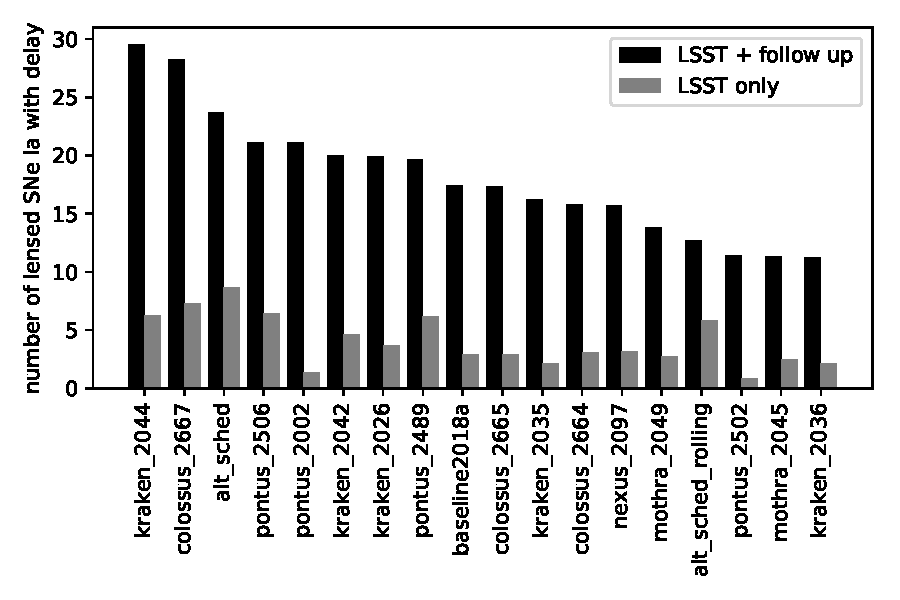
\includegraphics[scale=1]{sl_MetricLSST.pdf}
\caption{This plot quantifies 18 different cadence strategies for measuring time delays in LSNe Ia. The black bars consider LSST as a discovery machine in combination with follow-up observations in 3 filters (g,r,i) every second night. We assume follow-up observation would start 2 days after the third LSST data point in any filter exceeding the 5-$\sigma$ depth. For the grey bars only LSST data is used to measure time delays. Since for LSST only, the total numbers with good delays are very low, we advocate using LSST as a discovering machine with observational follow up. Therefore the black bars are the relevant ones to quantify different cadences. To summarize we are perfectly fine with a "baseline2018a" like cadence. To improve on this cadence longer cumulative seasonal lengths $\bar{t}_\mathrm{eff,cad}$, bigger survey areas $\Omega_\mathrm{cad}$ and a better sampling are helpful. On the other hand, rolling cadences are clearly disfavored despite the better sampling due to the substantially shortened cumulative seasonal length. }
\label{fig:final results}
\end{figure}

For the metric LSST data only we see that for the best strategies we will just have
a few systems where time-delay measurements are possible. Follow-up observations are therefore necessary to
increase the number of LSNe Ia with delays as visible which makes LSST + follow up the important metric to rank different observing strategies.

To summarize, for our science case of measuring time delays from as many lensed SNe as possible, it would be more effective to use LSST as a discovering machine with additional follow-up, instead of relying on LSST completely for the delay measurements. Therefore we are fine with the current baseline cadence. To improve on this cadence longer cumulative seasonal lengths $\bar{t}_\mathrm{eff,cad}$, bigger survey areas $\Omega_\mathrm{cad}$ and a more frequent sampling are helpful. The most important result from our investigation is that rolling cadences are clearly disfavored, because their shortened cumulative season lengths $\bar{t}_\mathrm{eff,cad}$ lead to overall a more negative impact on the number of LSNe Ia with delays, compared to the gain from the increased sampling frequency.
%of their shorter cumulative season lengths $\bar{t}_\mathrm{eff,cad}$ although they improve the sampling. Therefore we reject to improve on one of the 3 parameters our science case is mostly sensitive to, by worsen at the same time one of the others significantly. 
%

Further \cite{Goldstein:2018bue} performed detailed simulations of the gLSN population using a completely independent technique and pipeline and reached similar conclusions to the ones presented here: rolling cadences are strongly disfavored, and wide-area, long-season surveys with well sampled light curves are optimal.



\FloatBarrier
\subsection{Supernovae Lensed by Galaxy Clusters}
\textit{Contributors: Tanja Petrushevska}

Here, we focus on prospects of observing supernovae which are
lensed by known galaxy clusters. High-z galaxies that appear as
multiple images in the cluster field can host supernova
explosions. Strongly lensed supernovae by galaxy clusters not only
can be used as tools to examine both global cosmology, but also
the local environment of the cluster lenses. Cluster lensing time
scales are typically much longer and the microlensing effects are
almost negligible, which makes their measurement potentially more
feasible, especially if the lens potential is well studied and the
predicted time delays have small uncertainties. We calculate the
expected number of supernovae Ia in the multiply lensed background
galaxies by using the Hubble Frontier Fields cluster and Abell
1689. These clusters have been extensively studied, and given the
good quality data, well constrained magnification maps and time
delays can be obtained from the lensing models. We only considered
those that have a spectroscopic redshift. To obtain better image
depth, we combine the images that are taken closer than 5 days in
time. We note that these are a lower limits, since we have only
considered few clusters and the galaxies with spectroscopic
redshift. For this science case, the most important bands are i, z
and y. Since most of the light of nearby SNe is in the optical
bands, these filters are optimal for finding high-z SNe, as their
light is redshifted to the longer wavelengths. When we consider
the different observing strategies, we find that the rolling
cadences (mothra\_2045 and pontus\_2502) are disfavored given that
they do not return to the clusters as the other observing
strategies. The strategy pontus\_2489 provides slightly better
prospects compared to the others because it provides the most
number of visits to the same cluster fields.

\begin{figure}
\centering
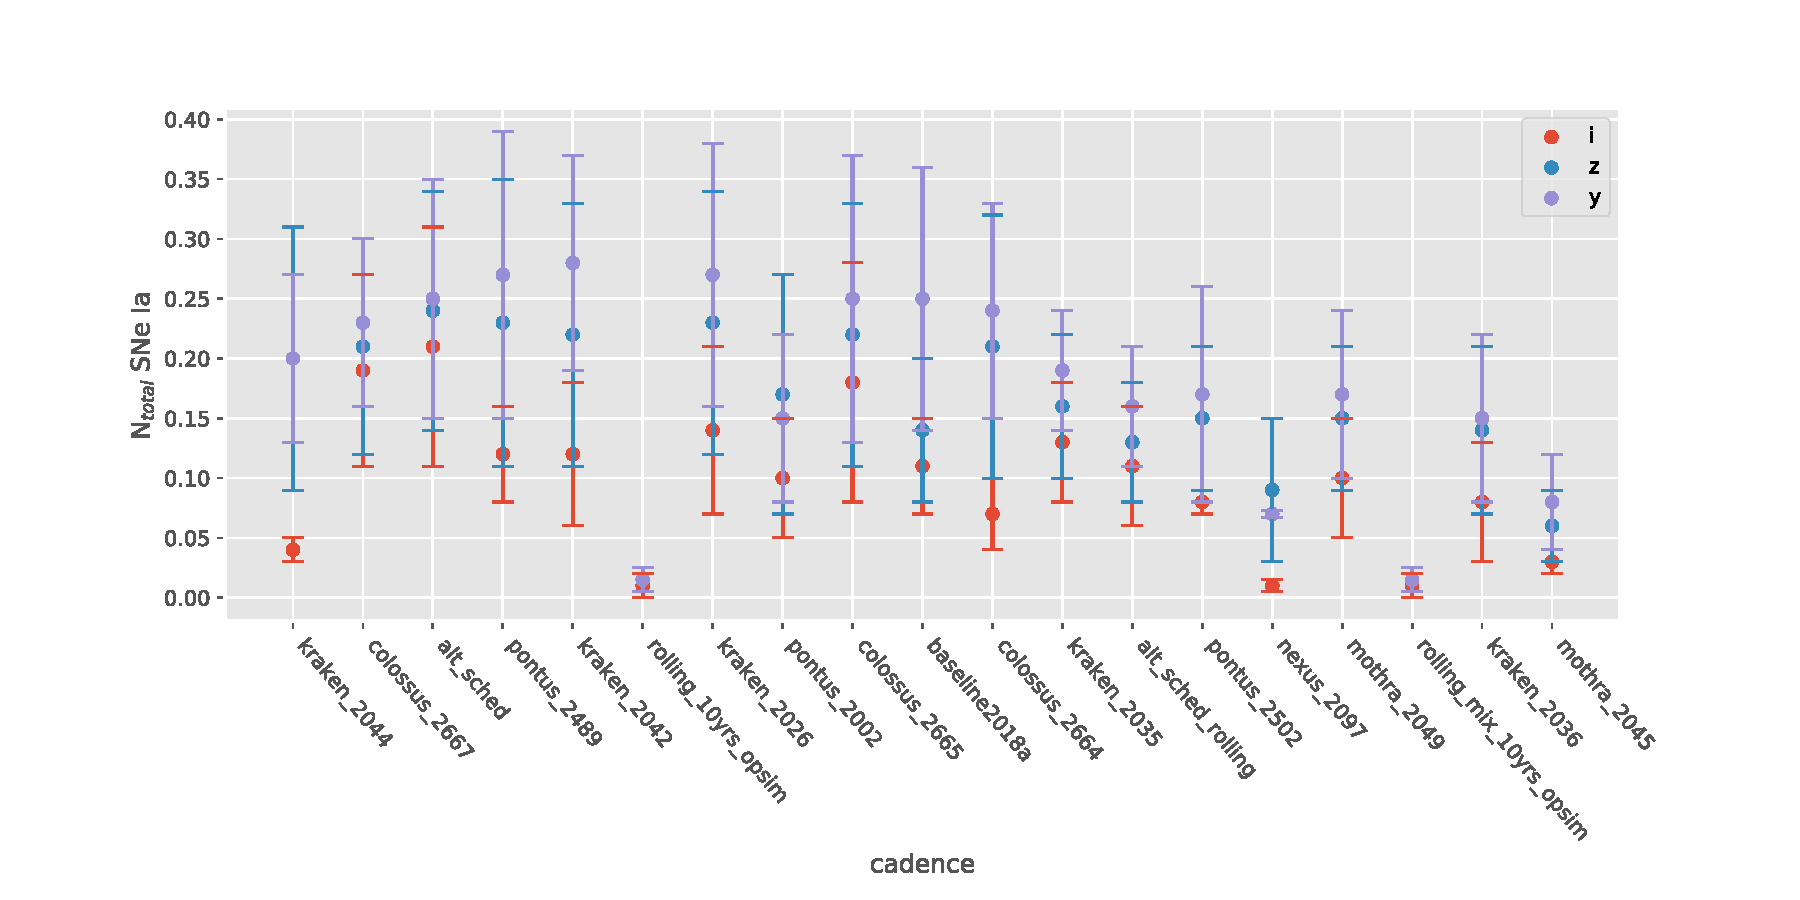
\includegraphics[scale=0.65]{figures/galaxy_lensing.pdf}
\caption{The expected total number of strongly lensed SNe Ia arising from the multiply imaged galaxies in the Hubble Frontier Fields and Abell 1689 in function of the observing strategy. \todo{Tanja}{include new cadences and do same estimates for CC SNe*}}
\end{figure}


\subsection{Lensed Quasars}
\textit{Contributors: TBD}



\FloatBarrier
\bibliography{../../Masterarbeit/Lit}

